\documentclass[a4paper]{article}

\usepackage{pgfplots}

\pgfplotsset{compat=1.5}

\begin{document}

%\tracingcommands=2\tracingmacros=2
{%
% THIS HERE IS AN EXTRACT OF THE MANUAL.

\pgfplotstableread{pgfplots.testplot}\plottable
\def\plot{%
	\begin{axis}[
		cell picture=false,anchor=north,
		width=5cm,
		name=test plot,
		xlabel=$x$,
		ylabel={$y$},% = \frac 12 \cdot x^3 - 4 x^2 -16 x$},
		legend style={at={(1.03,1)},anchor=north west},
		title=A test plot.
	]
		\addplot table from{\plottable};
		%\addplot coordinates {(0,0) (1,1)};
		\addlegendentry{$f(x)$}
		\addplot[red] plot[id=gnuplot_ppp,domain=-40:40,samples=120] gnuplot{10000*sin(x/3)};
		\addlegendentry{$g(x)$}
	\end{axis}
}%
\def\showit#1#2{%
	%\node[show them,#2] at (test plot.#1) {(s.#1)};
	\node[pin=#2:(s.#1),fill=black,circle,scale=0.3] at (test plot.#1) {};
}%
\tikzstyle{every pin}=[opacity=0.5,fill=yellow,rectangle,rounded corners=3pt,font=\tiny]%
		\begin{center}
			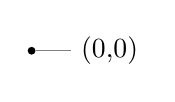
\begin{tikzpicture}
				\plot
				\showit{north}{90}
				\showit{north west}{135}
				\showit{west}{180}
				\showit{south west}{225}
				\showit{south}{270}
				\showit{south east}{305}
				\showit{east}{0}
				\showit{north east}{45}
				\showit{center}{90}
				
				\node[pin=0:{(0,0)},fill=black,circle,scale=0.3] at (0pt,0pt) {};
			\end{tikzpicture}
		\end{center}
Anchors on the outer bounding box,
		\begin{center}
			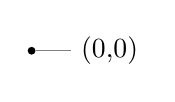
\begin{tikzpicture}
				\plot
				\showit{outer north}{90}
				\showit{outer north west}{135}
				\showit{outer west}{180}
				\showit{outer south west}{225}
				\showit{outer south}{270}
				\showit{outer south east}{305}
				\showit{outer east}{0}
				\showit{outer north east}{45}
				\showit{outer center}{90}
				\node[pin=0:{(0,0)},fill=black,circle,scale=0.3] at (0pt,0pt) {};
			\end{tikzpicture}
		\end{center}
There are anchors which have one coordinate on the outer bounding box, and one on the axis rectangle,
		\begin{center}
			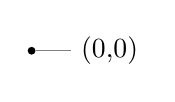
\begin{tikzpicture}
				\plot
				{\pgfplotsset{every pin/.append style={pin distance=1cm}}%
				\showit{above north}{90}
				}%
				\showit{above north east}{45}
				\showit{right of north east}{0}
				\showit{right of east}{0}
				\showit{right of south east}{0}
				\showit{below south east}{-45}
				{\pgfplotsset{every pin/.append style={pin distance=1cm}}%
				\showit{below south}{-90}
				}%
				\showit{below south west}{-135}
				\showit{left of south west}{180}
				\showit{left of west}{180}
				\showit{left of north west}{180}
				\showit{above north west}{135}
				\node[pin=0:{(0,0)},fill=black,circle,scale=0.3] at (0pt,0pt) {};
			\end{tikzpicture}
		\end{center}
And finally, we have origin anchors which are especially useful when axis lines pass through the origin,
		\begin{center}
			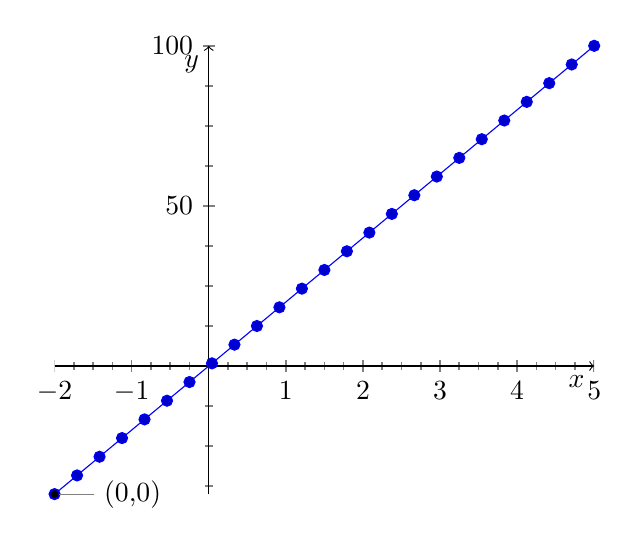
\begin{tikzpicture}
					\begin{axis}[
		cell picture=false,
						name=test plot,
						axis x line=center,
						axis y line=center,
						enlargelimits=false,
						minor tick num=3,
						tick style={semithick},
						tick align=center,
						xlabel=$x$,
						ylabel=$y$,
						every axis x label/.style={at={(current axis.right of origin)},anchor=north east},
						every axis y label/.style={at={(current axis.above origin)},anchor=north east},
						inner axis line style={->},
					]
					\addplot+[domain=-2:5] {20*x};
					\end{axis}
				{\pgfplotsset{every pin/.append style={pin distance=1cm}}%
				\showit{above origin}{45}
				}%
				\showit{right of origin}{45}
				{\pgfplotsset{every pin/.append style={pin distance=1cm}}%
				\showit{below origin}{0}
				}%
				\showit{left of origin}{135}
				\showit{origin}{135}
				\node[pin=0:{(0,0)},fill=black,circle,scale=0.3] at (0pt,0pt) {};
			\end{tikzpicture}
		\end{center}

}
\end{document}

